\documentclass{prova}

\usepackage{amsmath}
\usepackage{amsfonts}

\setlength{\textheight}{25cm}

\renewcommand{\sin}{\,\mbox{sen}\,}
\newcommand{\ds}{\displaystyle}

\professor{Prof.\@ Adriano Barbosa}
\disciplina{C\'alculo Diferencial e Integral III}
\avaliacao{P2}
\curso{Engenharia Civil}
\data{21/05/2021}

\begin{document}
	\cabecalho{5}  % o numero 5 indica a qnt de quadros na tabela de nota

    \textbf{Todas as respostas devem ser justificadas.}

    \begin{questionario}
	\q{Determine a largura e a altura do retângulo de perímetro $k$ e área
	   máxima.}
	\q{Calcule a integral dupla utilizando coordenadas polares $\ds
	   \int_0^{\sqrt{2}} \int_y^{\sqrt{4-y^2}} \frac{1}{\sqrt{1+x^2+y^2}}\ dx
	   dy$.}
	\q{Seja $E$ a região limitada pelos planos $y=x$, $x=0$, $z=0$ e pelo
	   cilíndro $y^2+z^2=1$. Calcule a integral $\iiint_E z\ dV$}
	   \begin{figure}[h]
	       \centering
               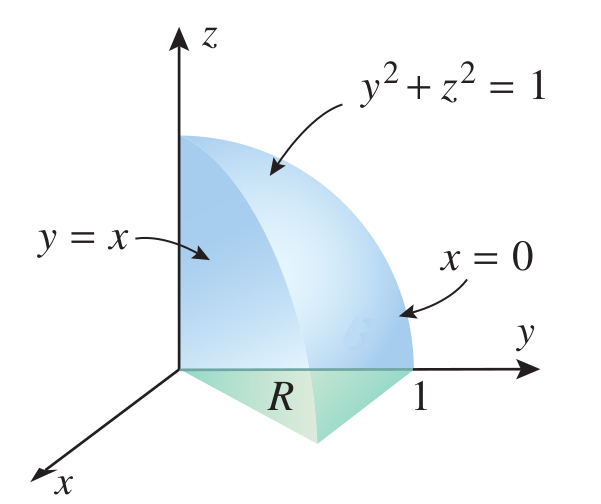
\includegraphics[width=0.3\textwidth]{regiaoE.png}
	       \qquad
               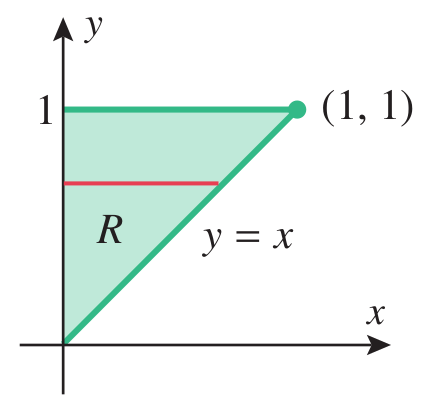
\includegraphics[width=0.25\textwidth]{regiaoR.png}
	   \end{figure}
	\q{Seja $F(x,y) = (2xy^3, 1+3x^2y^2)$:}
	   \begin{questionario}
	       \qq{Verifique se o campo é conservativo.}
	       \qq{Calcule a integral de linha $\ds\int_C F\cdot dr$, onde $C$
		   é o segmento de reta de $(3,1)$ até $(1,4)$.}
	       \qq{Calcule a integral de linha $\ds\int_C F\cdot dr$, onde $C$
		   é o segmento de reta de $(3,1)$ até $(0,0)$, seguido do
		   segmento de $(0,0)$ até $(1,7)$, seguido so segmento de
		   $(1,7)$ até $(1,4)$.}
           \end{questionario}
	\q{Sejam $C$ o retângulo com vértices em $(-2,1)$, $(4,1)$, $(4,2)$ e
	   $(-2,2)$ e $F(x,y) = (3xy, 2xy)$:}
	   \begin{questionario}
	       \qq{Verifique se as hipóteses do Teorema de Green são válidas.}
	       \qq{Calcule a integral $\int_C F\cdot dr$.}
	   \end{questionario}
    \end{questionario}
\end{document}
